%!TEX root=../document.tex

\section{Ergebnisse}
\label{sec:Ergebnisse}



\subsection{Projektaufbau}

\begin{minipage}{\linewidth}
	\centering
	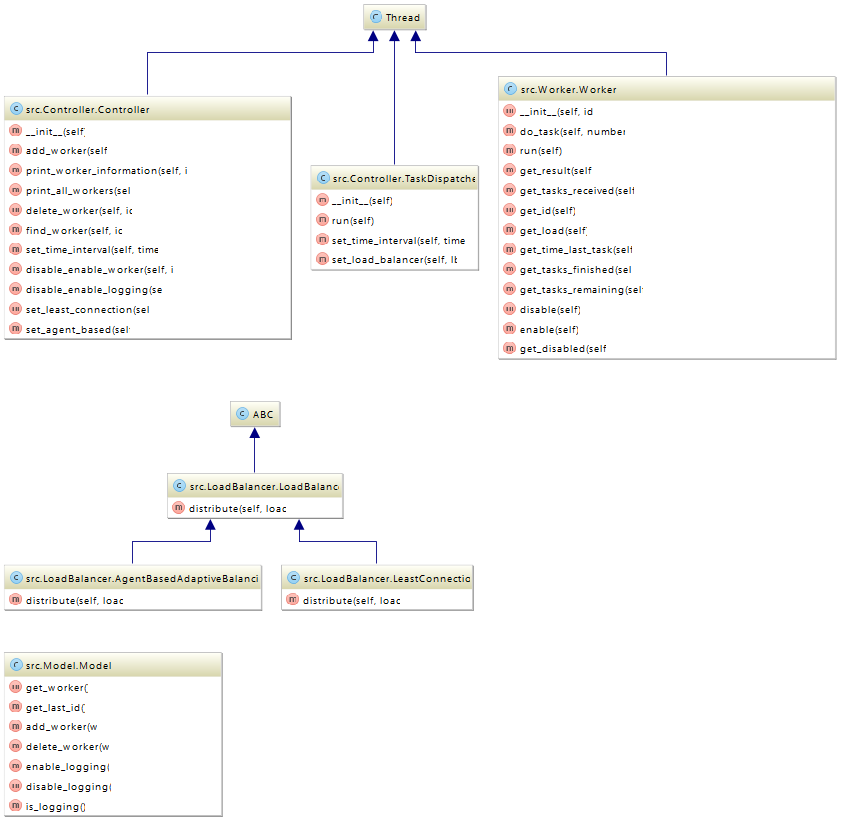
\includegraphics[width=1\linewidth]{images/class_diagram}
	\figcaption{Klassendiagramm}
\end{minipage}

Das Klassendiagramm zeigt die Relationen zwischen den einzelnen Klassen. 

\subsection{Controller}
Der Controller kümmert sich um die Instanziierung der Klassen und um die User-Eingaben.
Im Controller ist zusätzlich das User-Interface zu finden, welches in einer Endlosschleife User eingaben entgegennimmt und dem Controller übergibt und dieser dann an die zugehörigen Klassen weiterleitet.

\subsection{CLI Interface}
\begin{minipage}{\linewidth}
	\centering
	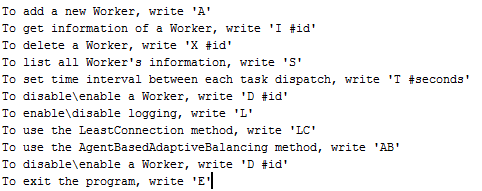
\includegraphics[width=0.8\linewidth]{images/cli_interface}
	\figcaption{Ein Command Line interface ist bereitgestellt für den User}
\end{minipage}

Der User kann folgende Tätigkeiten ausführen:

\begin{itemize}
	\item einen neuen \verb|Worker| hinzufügen
	\item die Information von einem bestimmten \verb|Worker| ausgeben
	\item einen \verb|Worker| löschen
	\item die Informationen von allen \verb|Worker| ausgeben
	\item den Zeit-Interval bestimmten in welchen die Tasks an den Load Balancer übergeben werden
	\item einen \verb|Worker| an oder ausschalten
	\item Logging an oder ausschalten
	\item die LeastConnection balancing methode verwenden
	\item die AgentBasedAdaptiveBalancing methode verwenden
	\item das Programm beenden
\end{itemize}

\subsection{Model}
Das Model hält alle relevanten Daten. Da es in Python keine statischen Klassen gibt, werden alle Methoden als statische methode mit der Annotation \verb|@staticmethod| versehen, um Zugriff auf die Funktionen ohne Instanziierung zu ermöglichen.

\subsection{TaskDispatcher}
Der TaskDispatcher ist ein Thread welcher alle x Sekunden einen Task an den \verb|LoadBalancer| sendet. Diese Klasse muss ein Thread sein da dieser parallel zu den anderen Klassen laufen muss um reibungslos einen praktischen Fall zu simulieren. 

In diesem Fall ist der Task lediglich eine immer um 1 inkrementierte Zahl welche anschließend vom \verb|Worker| abgearbeitet wird. 

\subsection{Worker}
Der Worker ist ein Thread, welcher Tasks in eine \verb|queue| übernimmt und diese dann Stück für Stück abarbeitet. Wie diese abgearbeitet wird, ist je nach Anwendungsfall anders. Z.B. könnte in einem realistischen Programm Verbindungen entgegenommen werden, welche anschließend Anfragen senden und vom Worker bearbeitet und zurückgesendet werden. 

In dem Fall wird von der Zahl, welche vom \verb|LoadBalancer| übergeben wurde, die Fakultät zu der davorigen Zahl dazu gerechnet. Grund für diese Berechnung ist einen Task darzustellen, welcher exponentiell immer länger dauert um tatsächlich den Sinn eines Load Balancers zu beweisen.

Um die Load Balancing Methoden implementieren zu können, muss der Worker bestimmte Statistiken bereitstellen können. Er muss bekannt geben können wieviele Aufgaben er bereits zugeteilt bekommen hat, und unter welcher Belastung er gerade steht. 

\subsubsection{get\_load()}
Diese Methode gibt aus, unter welcher Belastung der Arbeiter gerade steht. Der Worker besitzt das Attribut \verb|progress|, mit welchem mit der hilfe von \verb|desired_number| ausgerechnet werden kann zu wieviel Prozent der Task abgeschlossen wurde.

\begin{lstlisting}[language=python]
load = int((self.progress / self.desired_number) * 100)
\end{lstlisting}

Nun wird mit einem provisorischem Switch-Case überprüft ob der Arbeiter \verb|idle|, \verb|overloaded| oder \verb|disabled| ist. 

Falls der Arbeiter \verb|idle| ist, also momentan keinen Task abzuarbeiten hat, wird der Wert \textbf{0} zurückgegeben.

Falls der Arbeiter \verb|overloaded| ist, also noch zusätzliche Arbeit zu verrichten hat nach dem momentanen Task welcher abgearbeitet wird, wird der Wert \textbf{99} zurückgegeben. Es wird überprüft ob in der \verb|queue| mehr als 1 Wert vorhanden ist.

Falls der Arbeiter \verb|disabled| ist, also extern abgeschalten wurde, wird der Wert \textbf{101} zurückgegeben.


\begin{lstlisting}[language=python]
if load == 100:
return 0
elif self.is_disabled:
return 101
elif self.__q.qsize() > 1:
return 99
else:
return load
\end{lstlisting}
\subsection{LoadBalancer}
Da es in Python keine Interfaces gibt, wird die LoadBalancer klasse als \verb|Abstract Base Class|(ABC) definiert. Es wird die methode \verb|distribute()| vorgegeben, in welcher bereits Code für das Logging vorhanden ist und vererbt werden kann.

Im Grunde genommen geht es beim Load Balancer darum, dass anhand von bestimmten Kriterien (je nach Methode unterschiedlich) einem bestimmten Worker der Task zugeteilt wird. 

\subsubsection{LeastConnection}
Implementiert \verb|LoadBalancer|. Es wird die Methode \verb|distribute()| überschrieben, um die Funktionalität der Least Connection Methode zu implementieren.

\textbf{Diese Methode teilt jenem Worker den Task zu, welcher bisher die wenigstens Tasks zugeteilt bekommen hat.} 

\begin{lstlisting}[language=python]
determined_worker = min(Model.get_worker(), key=lambda x: x.get_tasks_received())
determined_worker.do_task(load)
\end{lstlisting}

\subsubsection{AgentBasedAdaptiveBalancing}
Laut folgender \underline{\textbf{\href{https://support.kemptechnologies.com/hc/en-us/articles/115005405746-API-for-Agent-Based-Adaptive-Balancing}{Seite}}} müssen folgende Bedingung gegeben sein vom Worker:

\begin{quote}
	Each server machine has to provide a file that contains a numeric value in the range between 0 and 102 representing the actual load on this server (0 = idle, 99 = overload, 101 = server down, 102 = administratively disabled).
\end{quote}

Nun wird dieser Wert nicht über ein File übergeben, sondern über \verb|get_load()|.

\textbf{Diese Methode teilt jenem Worker den Task zu, welcher momentan der niedrigsten Belastung untersteht.}

\begin{lstlisting}[language=python]
determined_worker = min(Model.get_worker(), key=lambda x: x.get_load())
\end{lstlisting}

Zusätzlich wird überprüft, falls jener Worker mit der niedrigsten \verb|load|, eine load von \verb|99| oder \verb|101| besitzt, bedeutet dies dass jeder Server überlastet bzw. abgeschalten ist!

\begin{lstlisting}[language=python]
if determined_worker.get_load() == 101 or determined_worker.get_load() == 99:
print(''Task was dismissed because all Workers are overloaded or disabled!'')
return
else:
determined_worker.do_task(load)
\end{lstlisting}

\subsection{Belastungstests}
Es wurde beim Logging die CPU-Usage, die generelle RAM-Usage und die RAM-Usage vom Programm hinzugefügt. Dafür wurde das Package \verb|psutil verwendet|:

\begin{lstlisting}[language=python]
print(''CPU Usage: '' + str(psutil.cpu_percent()))
print(''General RAM Usage: '' + str(psutil.virtual_memory()))  # physical memory usage
pid = os.getpid()
py = psutil.Process(pid)
memoryUse = py.memory_info()[0] / 2. ** 30  # memory use in GB
print('Process RAM Usage: ', memoryUse)
\end{lstlisting}

\begin{minipage}{\linewidth}
	\centering
	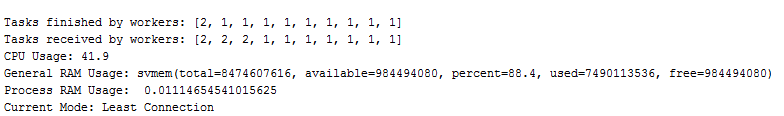
\includegraphics[width=1\linewidth]{images/belastung}
	\figcaption{Belastungstest von CPU und RAM}
\end{minipage}

Es ist zu erkennen, je länger das Programm läuft desto mehr RAM wird verbraucht vom Programm.

\begin{minipage}{\linewidth}
	\centering
	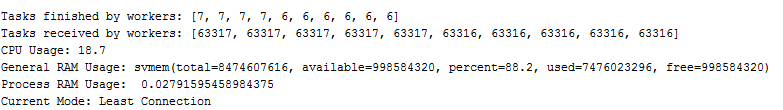
\includegraphics[width=1\linewidth]{images/belastung2}
	\figcaption{Belastungstest von CPU und RAM nach längerer Belastung}
\end{minipage}

Zu beachten: es wurde die Least Balancing Methode verwendet, deswegen wurde einige Mehr tasks zugeteilt als abgearbeitet. Darauf ist zurückzuführen dass mehr RAM in Verwendung ist, da jeder einzelner Worker den Task in der \verb|queue| speichern muss, was natürlich im RAM Speicher verbraucht. 

\subsection{Konkrete Fragestellungen}
\subsubsection{Vergleichen Sie die verwendeten Load Balancing Methoden und stellen Sie diese gegenüber.}
Der Vergleich ist zu sehen, wenn man sich anschaut welchen Workern wieviele Tasks zugewiesen wurden:

\begin{table}[h!]
	\centering
	\begin{tabular}{c c}
		\begin{minipage}{.5\textwidth}
			\centering
			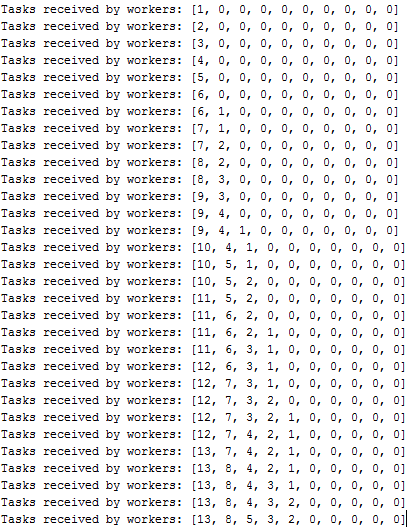
\includegraphics[width=\linewidth]{images/AB}
			\figcaption{Agent Based Adaptive Balancing}
		\end{minipage}
		
		&
		\begin{minipage}{.5\textwidth}
			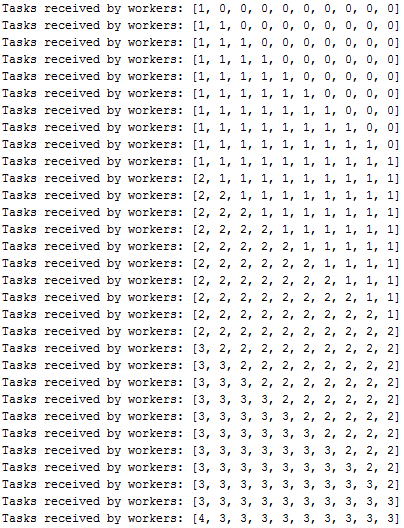
\includegraphics[width=\linewidth]{images/LC}
			\figcaption{Least Connection Balancing}
		\end{minipage}
		
		\\
	\end{tabular}
\end{table}

Es wurden \textbf{31} Tasks auf \textbf{10} Worker vom jeweiligen LoadBalancer verteilt:

Es ist zu sehen, dass das Agent Based Adaptive Balancing anfänglich nur einem Worker Tasks zuteilt. Dies liegt daran, dass die Tasks exponentiell länger werden und am Anfang sehr schnell abgearbeitet werden können. Erst wenn die Tasks länger zum abarbeiten brauchen, werden sie auch auch anderen Workern zugeilt.

Beim Least Connection Balancing ist die Funktionsweise klar zu sehen: Es wird systematisch den jeweiligen Arbeitern die Arbeit zugeteilt. Problem dabei besteht darin, dass beim Verteilen nicht auf die Belastung der einzelnen Arbeiter geachtet wird, das bedeutet dass wenn ein Arbeiter einen sehr aufwendigen Task zugeteilt bekommt, erhält er trotzdem gleich schnell wieder einen task wie jener Worker der einen sehr schnell abgearbeiteten Task zugeteilt bekommen hat.
\subsubsection{Was kann als Gewichtung bei Weighted Round Robin verwendet werden?}
Mit der Gewichtung geht es darum, welchem Server mehr oder weniger Tasks zugewiesen werden. Dabei geht es um Hardware-Spezifikationen (\textbf{Performance}), beispielsweise besitzt ein Server mit mehr RAM eine höhere Gewichtung als einer mit weniger Hauptspeicher.
In den meisten Fällen wird geachtet auf:

\begin{itemize}
	\item RAM
	\item CPU
	\item HDD oder SSD
	\item Übertragungsrate
\end{itemize}

\subsubsection{Warum stellt die Hochverfügbarkeit von IT Systemen in der heutigen Zeit eine sehr wichtige Eigenschaft dar?}
In einer Zeit wo Steuererklärungen und Banküberweisungen über das Internet ablaufen, müssen Webapplikationen immer zuverlässig verfügbar sein. Zusätzlich durch das immer mehr populär werdende Online-Shopping werden sehr viele User-Anfragen an die Server gestellt, welche alle \textbf{zuverlässig} und \textbf{schnell} bearbeiten werden müssen.
\subsubsection{Welche anderen Massnahmen neben einer Lastverteilung müssen getroffen werden, um die ''Hochverfügbarkeit'' sicher zu stellen?}
Natürlich müssen genug Server zur Verfügung stehen, der beste Lastverteilungssystem ist unbrauchbar wenn es nichts gibt auf was die Last verteilt werden kann. Es muss auch die interne und die Verbindung mit dem Internet gewährleistet sondern, Kommunikation ist das wichtigste!
\subsubsection{Was versteht man unter Session Persistenz und welche Schwierigkeiten ergeben sich damit?}
Eine Lastverteilungsmethode bei welcher der Load Balancer die gesamte session information während der Applikationstransaktion speichern muss. Falls die Sitzung abbricht aus unerwarteten Gründen, kann es zu fatalen Datenverlusten kommen.
\subsubsection{Nennen Sie jeweils ein Beispiel, wo Session Persistenz notwendig bzw. nicht notwendig ist.}
Notwendig ist es bei Webanwendungen welche eine Sitzung aufbauen müssen. Es ist zum Beispiel auf \textbf{Amazon.de} nötig, ab dem Moment wo ein Artikel zum Warenkorb hinzugefügt oder man sich einloggt.

Nicht benötigt wird es bei Seiten welche lediglich eine Aufgabe erledigen und keine Sitzung aufbauen müssen, beispielsweise ein RGB-to-HEX Converter.
\subsubsection{Welcher Unterschied besteht zwischen einer ''server-side'' bzw ''client-side''\\ Lastverteilungslösung?}
Beim Client-seitigen Load Balancer ist lokal ein Register vorhanden, in welchem alle Services mit den jeweiligen Informationen bereitstehen. Bei einer Anfrage wird der URL des passenden Services abefragt.

Beim Server-seitigen Load Balancer ist eine zentrale Komponente vorhanden, welche alle Clients/Tasks zu den passenden Server/Abarbeitungskomponente verweist. 
\subsubsection{Was versteht man unter dem ''Mega-Proxy-Problem''?}
Die Mega Proxy Session, auch bekannt als Mega Proxy Problem, beschreibt jene Situation in welcher die IP des Users nicht korrekt herausgefunden werden kann. Dieses Problem tritt auf wenn die User hinter einem sogenannte Proxy-Server stehen, welcher die IP-Adresse des Users zu der des Proxy-Servers ändert. Grund für die Verwendung eines Proxy-Server ist der Wunsch von Anonymität bzw. Netz-Sicherheit.
